\section{Background}\label{sec:background}
In this section, we provide an overview of the preprocessing techniques and machine learning models used in our proposed pipeline. 
We outline the various normalization techniques and dimensionality reduction methods, followed by the ensemble learning, linear models, and regularization models used.
Finally, we outline stacked generalization. 

\subsection{Preprocessing}
In this subsection, we discuss the preprocessing methods used in our machine learning pipeline.
We cover various normalization techniques such as Z-score normalization, max absolute scaling, min-max normalization, robust scaling, Norm 3, power transformation, and quantile transformation.
These techniques are essential for standardizing data, handling different scales, and improving the performance of machine learning models.

\subsubsection{Z-score Normalization}
Z-score normalization, also standardization, transforms data to have a mean of zero and a standard deviation of one.
This technique is useful when the actual minimum and maximum of a feature are unknown or when outliers may significantly skew the distribution.
The formula for Z-score normalization is given by:

$$
v' = \frac{v - \overline{F}}{\sigma_F},
$$

where $v$ is the original value, $\overline{F}$ is the mean of the feature $F$, and $\sigma_F$ is the standard deviation of $F$.
By transforming the data using the Z-score, each value reflects its distance from the mean in terms of standard deviations.
Z-score normalization is particularly advantageous in scenarios where data features have different units or scales, or when preparing data for algorithms that assume normally distributed inputs~\cite{dataminingConcepts}.

\subsubsection{Max Absolute Scaler}
Max absolute scaling is a normalization technique that scales each feature individually so that the maximum absolute value of each feature is 1.
This results in the data being normalized to a range between -1 and 1.
The formula for max absolute scaling is given by:
$$
	X_{\text{scaled}} = \frac{x}{\max(|x|)},
$$
where $x$ is the original feature value and $X_{\text{scaled}}$ is the normalized feature value.
This scaling method is useful for data that has been centered at zero or data that is sparse, as max absolute scaling does not center the data.
This maintains the sparsity of the data by not introducing non-zero values in the zero entries of the data~\cite{Vasques2024}.

\subsubsection{Min-Max Normalization}\label{subsec:min-max}
Min-max normalization rescales the range of features to $[0, 1]$ or $[a, b]$, where $a$ and $b$ represent the new minimum and maximum values, respectively.
The goal is to normalize the range of the data to a specific scale, typically 0 to 1.
Mathematically, min-max normalization is defined as:
$$
	v' = \frac{v - \min(F)}{\max(F) - \min(F)} \times (b - a) + a,
$$
where $v$ is the original value, $\min(F)$ and $\max(F)$ are the minimum and maximum values of the feature $F$, respectively.

This type of normalization is beneficial because it ensures that each feature contributes equally to the analysis, regardless of its original scale.

\subsubsection{Robust Scaler}
The robust scaler is a normalization technique that removes the median and scales the data according to the quantile range.
The formula for the robust scaler is given by:
$$
X_{\text{scaled}} = \frac{X - \text{Q1}(X)}{\text{Q3}(X) - \text{Q1}(X)} \: ,
$$
where $X$ is the original data, $\text{Q1}(X)$ is the first quartile of $X$, and $\text{Q3}(X)$ is the third quartile of $X$.
This technique can be advantageous in cases where the data contains outliers, as it relies on the median and quantile range instead of the mean and variance, both of which are sensitive to outliers~\cite{Vasques2024}.

\subsubsection{Norm 3}
As previously mentioned, the \gls{chemcam} instrument consists of three spectrometers, each producing 2048 channels.
For data normalization, we follow the approach taken by the ChemCam team and normalize across individual spectrometers' wavelength ranges, a process known as \textit{Norm 3}~\cite{cleggRecalibrationMarsScience2017, andersonImprovedAccuracyQuantitative2017}.
This method ensures that the wavelength intensities captured by each spectrometer are normalized independently, thus preserving the relative intensities within each spectrometer.

Figure~\ref{fig:spectral_plot} shows a spectral plot of the \gls{ccs} data for the \textit{ultramafic} sample, illustrating the three distinct spectral regions, each captured by one of the three spectrometers.
Specifically, one spectrometer captures the \gls{uv} region, another captures the \gls{vio} region, and the third captures the \gls{vnir} region.

\begin{figure}[H]
	\centering
	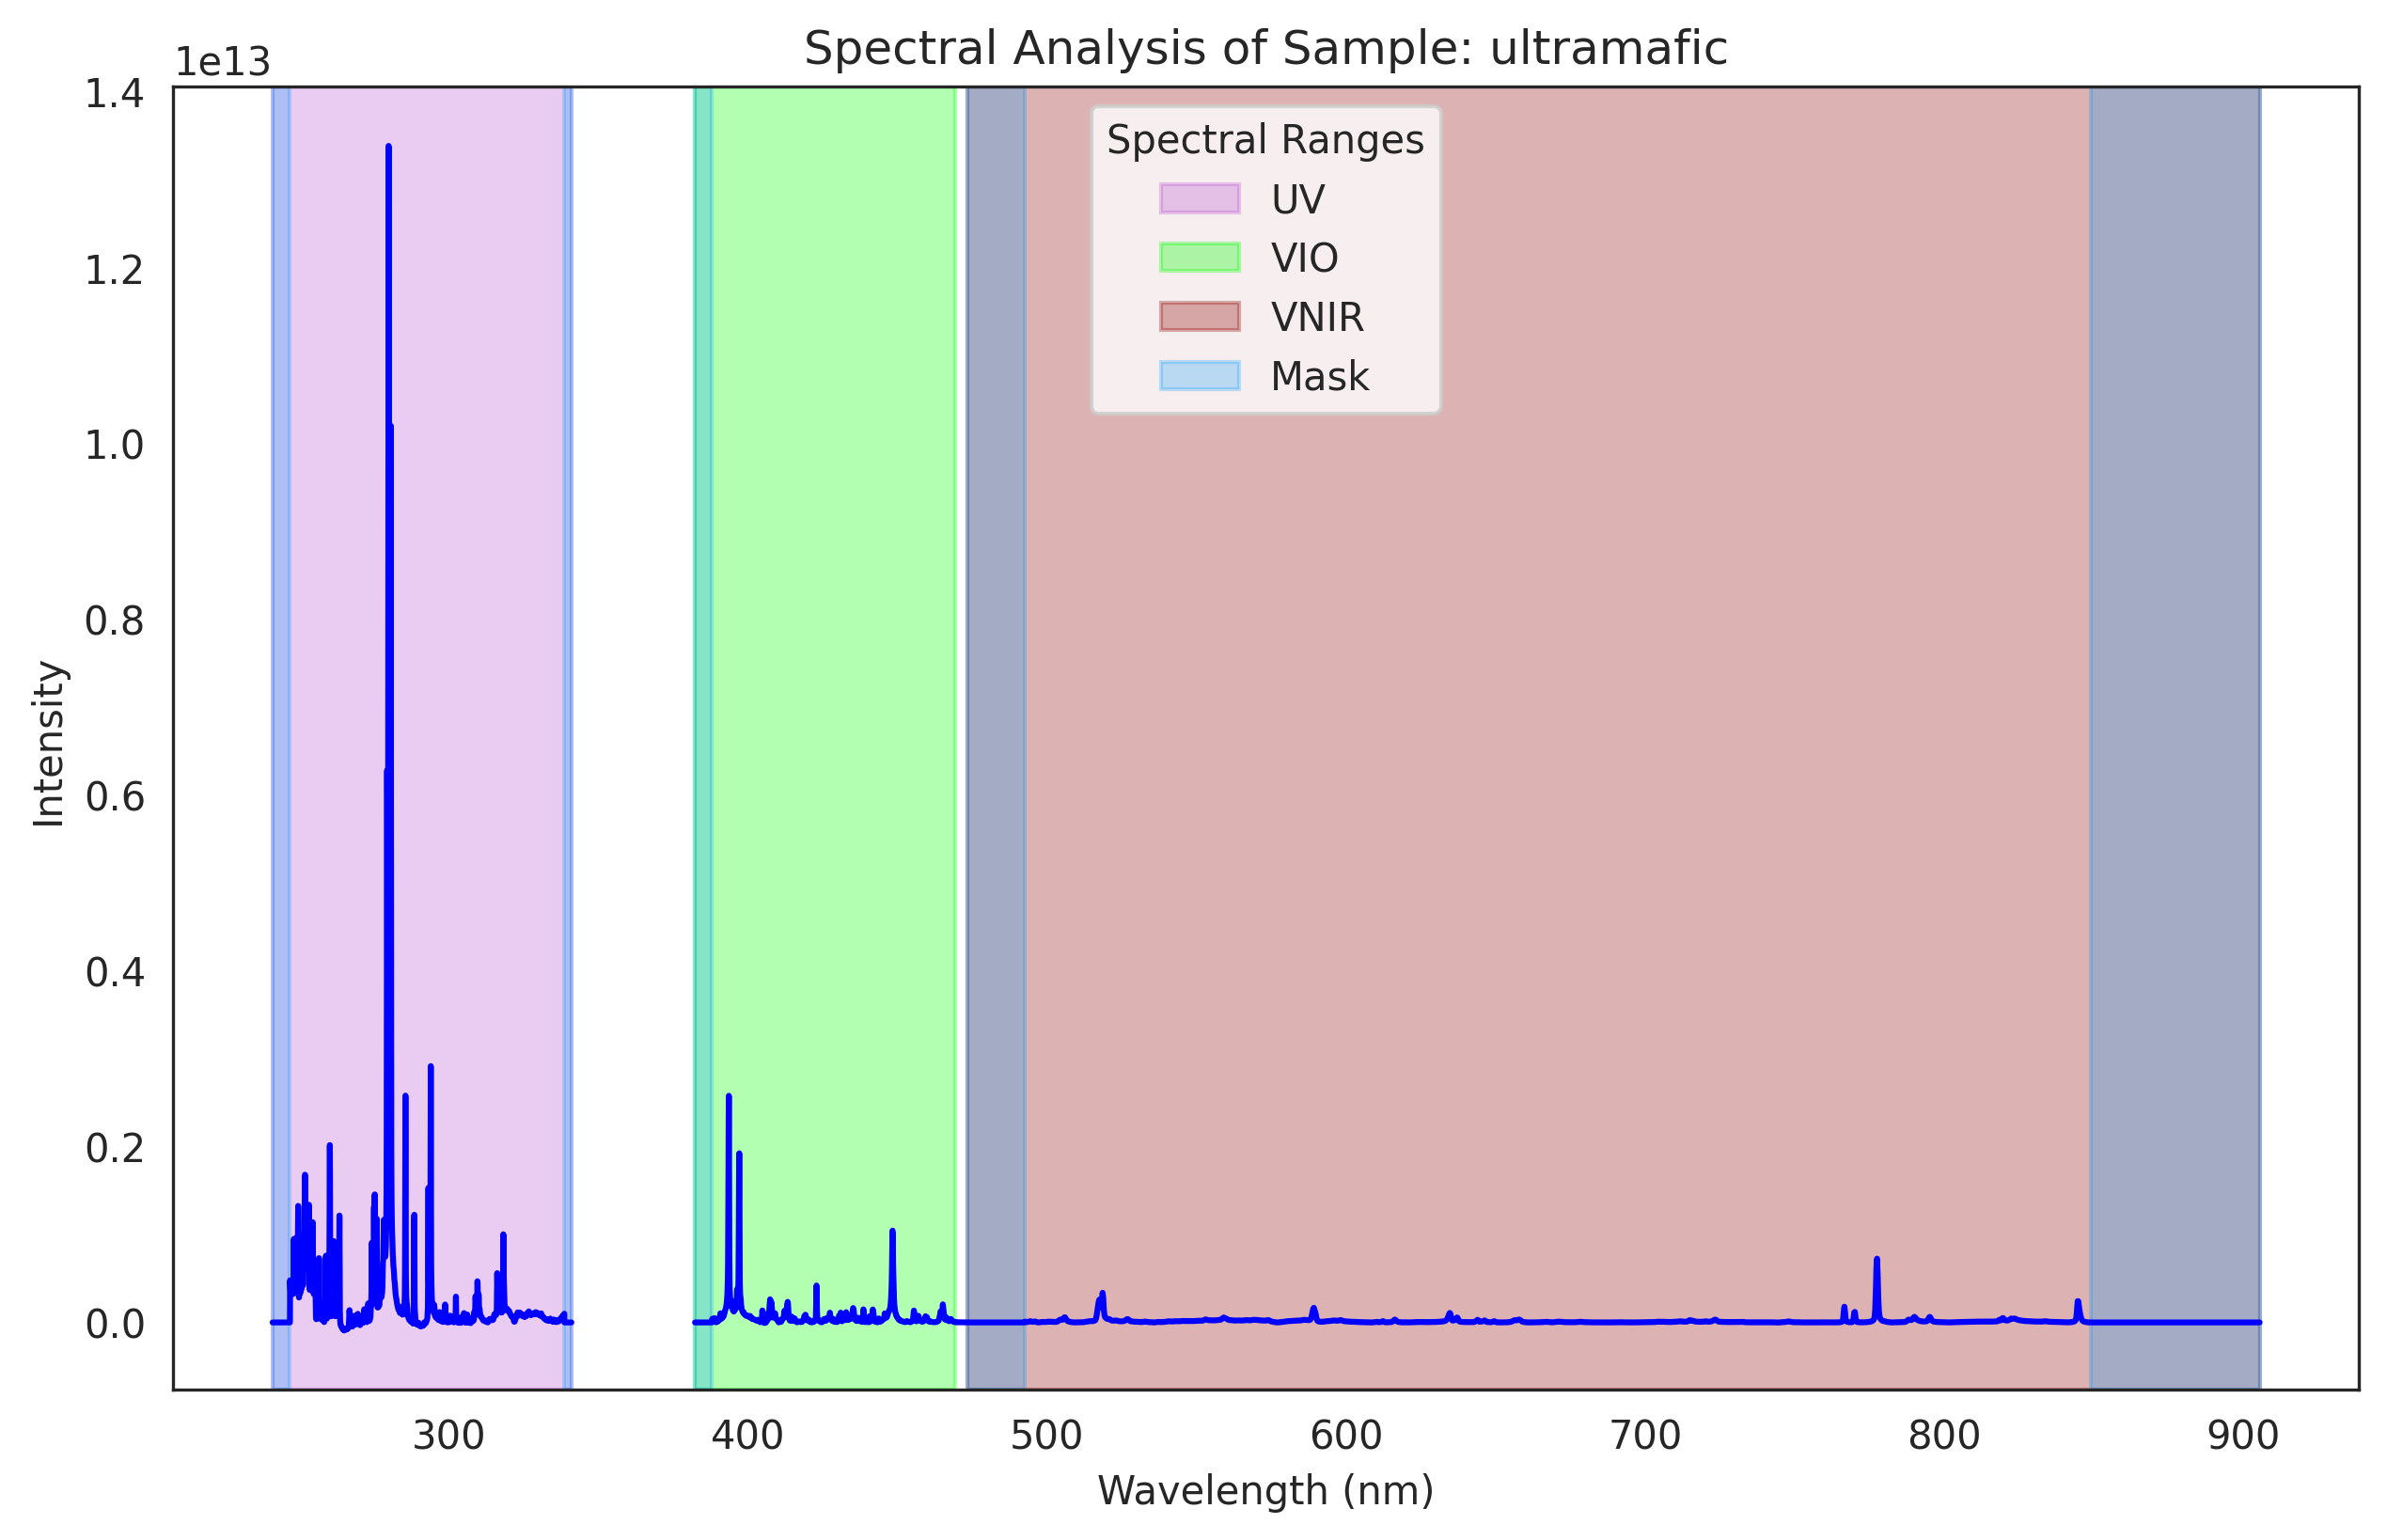
\includegraphics[width=0.5\textwidth]{images/spectral_plot.png}
	\caption{Spectral plot of the \gls{ccs} data for the \textit{ultramafic} sample. The wavelengths represent the spectral channels.}
	\label{fig:spectral_plot}
\end{figure}

Formally, Norm 3 is defined as

\begin{equation}
	\tilde{X}_{i,j}^{(\gamma)} = \frac{X_{i,j}^{(\gamma)}}{\sum_{j=1}^{N} X_{i,j}^{(\gamma)}},
\end{equation}

where

\begin{itemize}
	\item $\tilde{X}_{i,j}^{(\gamma)}$ is the normalized wavelength intensity for the $i$-th sample in the $j$-th channel on the $\gamma$-th spectrometer, with $\gamma \in \{1, 2, 3\}$ representing the \gls{uv}, \gls{vio}, and \gls{vnir} spectrometers, respectively,
	\item $X_{i,j}^{(\gamma)}$ is the original wavelength intensity for the $i$-th sample in the $j$-th channel on the $\gamma$-th spectrometer, and
	\item $N = 2048$ is the number of channels in each spectrometer.
\end{itemize}

This normalization method results in a total of $3N = 6144$ normalized features for each sample, as each of the three spectrometers contributes 2048 channels.

\subsubsection{Power Transformation}
Power transformations are a class of mathematical functions used to stabilize variance and make data more closely approximate a normal distribution.
They are particularly useful in statistical modeling and data analysis to meet the assumptions of linear models.

One of the first influential power transformation techniques is the Box-Cox power transform, introduced by \citet{BoxAndCox} in 1964.
This is defined for positive data and is aimed at normalizing data or making it more symmetric. The transformation is given by:

$$
\text{BC}(\lambda, x) =
\begin{cases}
\frac{x^\lambda - 1}{\lambda} & \text{if } \lambda \neq 0 \\
\log(x) & \text{if } \lambda = 0
\end{cases}
$$
where $ \lambda $ is the transformation parameter and $x$ is the input data.
$\lambda$ determines the extend and nature of the transformation, where positive values of $\lambda$ apply a power transformation and $\lambda = 0$ applies a logarithmic transformation.

To overcome the limitations of the Box-Cox transformation, \citet{YeoJohnson} introduced a new family of power transformations that can handle both positive and negative values.
The Yeo-Johnson power transformation is defined as:

$$
y =
\begin{cases}
\frac{((x + 1)^\lambda - 1)}{\lambda} & \text{for } x \geq 0, \lambda \neq 0 \\
\log(x + 1) & \text{for } x \geq 0, \lambda = 0 \\
-\frac{((-x + 1)^{2 - \lambda} - 1)}{2 - \lambda} & \text{for } x < 0, \lambda \neq 2 \\
-\log(-x + 1) & \text{for } x < 0, \lambda = 2
\end{cases}
$$
where $x$ is the input data, $y$ is the transformed data, and $\lambda$ is the transformation parameter.
For non-negative values, the Yeo-Johnson transformation simplifies to the Box-Cox transformation, making them equivalent in this context.
The key benefit of the Yeo-Johnson transformation is its ability to handle any real number, making it a robust choice for transforming data to achieve approximate normality or symmetry.
This property is particularly beneficial for preparing data for statistical analyses and machine learning models that require normally distributed input data.

\subsubsection{Quantile Transformer}
Quantile transformation is a method that applies a non-linear transformation to map data to a uniform or normal distribution.
This process involves mapping the data $X$ to a set of probabilities $p$ using the \gls{cdf}, which indicates the probability that a random variable will be less than or equal to a specific value in $X$'s original distribution.
Subsequently, the quantile function, which is the inverse of the \gls{cdf} of the desired distribution, is applied to these probabilities $p$ to generate the transformed data.
This method forces the data to conform to the specified distribution regardless of the original distribution's form~\cite{Vasques2024}.

\subsubsection{Principal Component Analysis (PCA)}\label{subsec:pca}
\gls{pca} is a dimensionality reduction technique that transforms a set of possibly correlated variables into a smaller set of uncorrelated variables called \textit{principal components}.
We give an overview of the \gls{pca} algorithm based on \citet{James2023AnIS}.

First, the data matrix $\mathbf{X}$ is centered by subtracting the mean of each variable to ensure that the data is centered at the origin:

$$
\mathbf{\bar{X}} = \mathbf{X} - \mathbf{\mu},
$$

where $\mathbf{\bar{X}}$ is the centered data matrix and $\mathbf{\mu}$ is the mean of each variable.

The covariance matrix of the centered data is then computed:

$$
\mathbf{C} = \frac{1}{n-1} \mathbf{\bar{X}}^T \mathbf{\bar{X}},
$$

where $n$ is the number of samples.

Then, the covariance matrix $\mathbf{C}$ is decomposed into its eigenvectors $\mathbf{V}$ and eigenvalues $\mathbf{D}$:

$$
\mathbf{C} = \mathbf{V} \mathbf{D} \mathbf{V}^T,
$$

where $\mathbf{V}$ contains the eigenvectors of $\mathbf{C}$. 
These eigenvectors represent the principal components, indicating the directions of maximum variance in $\mathbf{X}$. 
The interpretation of the principal components is that the first captures the most variance, the second captures the next most variance, and so on. 
The matrix $\mathbf{D}$ is diagonal and contains the eigenvalues, each quantifying the variance captured by its corresponding principal component.

These components are the scores $\mathbf{T}$, calculated as follows:

$$
\mathbf{T} = \mathbf{\bar{X}} \mathbf{V}_n,
$$

where $\mathbf{V}_n$ includes only the top $n$ eigenvectors.
The scores $\mathbf{T}$ are the new, uncorrelated features that reduce the dimensionality of the original data, capturing the most significant patterns and trends.

Finally, the original data points are projected onto the space defined by the top $n$ principal components, which transforms $X$ into a lower-dimensional representation:

$$
\mathbf{X}_{\text{reduced}} = \mathbf{\bar{X}} \mathbf{V}_n,
$$

where $\mathbf{V}_n$ is the matrix that only contains the top $n$ eigenvectors.

\subsubsection{Kernel PCA}
We provide a brief overview of the \gls{kernel-pca} algorithm based on \citet{learningwithkernels}.
\gls{kernel-pca} is an extension of traditional \gls{pca} designed to handle nonlinear relationships among data points.
The core idea behind \gls{kernel-pca} is to map data into a higher-dimensional space using a kernel function, a technique known as the kernel trick.
This mapping enables linear separation of data points in the higher-dimensional space, even if they are not linearly separable in the original space.

Similar to \gls{pca}, as described in Section~\ref{subsec:pca}, the goal of \gls{kernel-pca} is to extract the principal components of the data.
However, unlike \gls{pca}, \gls{kernel-pca} does not compute the covariance matrix of the data directly, as it often is infeasible to compute for high-dimensional datasets.
\gls{kernel-pca} instead leverages the kernel trick to computate the similarities between data points directly in the original space using a kernel function $k(\mathbf{x}_i, \mathbf{x}_j)$.
This kernel function implicitly computes the dot product $\Phi(\mathbf{x}_i)^\top \Phi(\mathbf{x}_j)$ in the higher-dimensional feature space without explicitly performing the mapping.
By constructing a kernel matrix $\mathbf{K}$ using these pairwise similarities, \gls{kernel-pca} can perform eigenvalue decomposition to obtain the principal components in the feature space, similar to regular \gls{pca} as described in Section~\ref{subsec:pca}.
However, in \gls{kernel-pca}, the eigenvalue decomposition is performed on the kernel matrix $\mathbf{K}$ rather than the covariance matrix $\mathbf{C}$.

\subsection{Ensemble Learning Models}
In this section we introduce the concept of ensemble learning and decision trees based on \citet{James2023AnIS}, as they are fundamental aspects of the ensemble learning models we discuss.
Following this, we outline \gls{etr}, \gls{gbr}, \gls{ngboost}, and \gls{xgboost}.

\subsubsection{Ensemble Learning}
Ensemble learning is a technique in machine learning where multiple models, known as \textit{weak learners}, are combined to produce more accurate predictions.
Mathematically, ensemble learning can be defined as combining the predictions of $M$ weak learners to form a final prediction $\hat{y}$, such that:
\begin{equation}
    \hat{y} = \sum_{m=1}^{M} \alpha_m \hat{y}_m,
\end{equation}
where $\hat{y}_m$ is the prediction of the $m$-th weak learner and $\alpha_m$ is the weight assigned to the $m$-th weak learner.
While there are various choices for weak learners, decision trees are a common choice\cite{James2023AnIS}.

\subsubsection{Decision Trees}
A decision tree is a supervised learning model that partitions data into subsets based on feature values, creating a tree structure.
The goal is to create a tree that predicts the target variable by dividing the data into increasingly homogeneous subsets.
Each internal node in the tree represents a decision based on a specific feature, while each leaf node represents a prediction for the target variable.
The tree can make predictions for new data points by following a path from the root to a leaf node\cite{James2023AnIS}.

\subsubsection{Extra Trees Regressor (ETR)}
We give an overview of \gls{rf} based on \citet{James2023AnIS}.
Then, we introduce the \gls{etr} model based on \citet{geurtsERF}.

\gls{rf} is an ensemble learning method that improves the accuracy and robustness of decision trees by building multiple trees and combining their predictions.
Each tree is trained on a random subset of the data using bootstrap sampling, where samples are drawn with replacement, meaning the same sample can be selected multiple times.
This introduces variability and reduces overfitting, as some data points may appear multiple times while others may be omitted.
By aggregating predictions from multiple trees, the model achieves better generalization and robustness.

Mathematically, the prediction of a \gls{rf} model can be represented as:

$$
f(x) = \frac{1}{M} \sum_{m=1}^{M} f_m(x),
$$

where $f_m(x)$ is the prediction of the $m$-th tree, and $M$ is the total number of trees.

\gls{etr} extends the \gls{rf} model by introducing additional randomness in the tree-building process, specifically through random feature selection and random split points.
While \gls{rf} uses bootstrap sampling and selects the best split from a random subset of features to create a set of diverse samples, \gls{etr} instead selects split points randomly within the chosen features, introducing additional randomness.
This process results in even greater variability among the trees, aiming to reduce overfitting and improve the model's robustness.
As a tradeoff, \gls{etr} is less interpretable than a single decision tree, as the added randomness can introduce more bias than \gls{rf}.
However, it often achieves better generalization performance, especially in high-dimensional or noisy datasets.

\subsubsection{Gradient Boosting Regression (GBR)}\label{sec:gradientboost}
In this section, we introduce \gls{gbr} primarily based on \citet{hastie_elements} and \citet{burkovHundredpageMachineLearning2023}.

Gradient Boosting is a machine learning technique used for various tasks, including regression and classification.
The fundamental concept involves sequentially adding models to minimize a loss function, where each successive model addresses the errors of the ensemble of preceding models.

This technique utilizes gradient descent to optimize the loss function, allowing for the selection of different loss functions depending on the specific task.
\gls{gbr} is a specialized application of gradient boosting for regression tasks, where it minimizes a regression-appropriate loss function, such as mean squared error or mean absolute error.

The process starts with an initial model $f_{0}(x)$ that minimizes the loss function over the entire dataset:
$$
f_{0}(x)=\arg\min_{\gamma}\sum^{N}_{i=1}L(y_{i},\gamma)
$$
where $L(y,\hat{y})$ is the chosen loss function, $N$ is the number of samples, $y_{i}$ are the true values, and $\gamma$ is a constant.

Then we start the iterative process of adding models to the ensemble.
For each iteration $m$, from $1$ to $M$:

\begin{enumerate}
    \item Compute the residuals of the current model. For regression, this could be the squared error loss, $L(y, \hat{y}) = (y - \hat{y})^2$. The residuals $r_{i}^{(m)}$ for each data point $i$ are calculated as $r_{i}^{(m)} = y_{i} - f_{m-1}(x_{i})$, where $f_{m-1}(x_{i})$ is the prediction of the previous model.
    \item Fit a new model $h_{m}(x)$ to the residuals. This model aims to correct the errors of the current ensemble by using the residuals instead of ground truth values. Essentially, $h_{m}(x)$ tries to predict the residuals $r_{i}^{(m)}$.
    \item Update the ensemble model by adding the predictions of the new model $h_{m}(x)$, multiplied by a learning rate $\eta$. The learning rate $\eta$ controls the contribution of each new model to the ensemble, preventing overfitting by scaling the updates:
    $$
    f_{m}(x)=f_{m-1}(x)+\eta h_{m}(x)
    $$
\end{enumerate}

This iterative process continues until the maximum number $M$ of trees are combined, resulting in the final model $\hat{f}(x) = f_{M}(x)$.

\subsubsection{Natural Gradient Boosting (NGBoost)}
\gls{ngboost} is a variant of the gradient boosting algorithm that leverages the concept of natural gradients with the goal of improving convergence speed and model performance.
In more complex models, the parameter space can be curved and thus non-Euclidean, making the standard gradient descent less effective.
Consequently, using the standard gradient descent can lead to slow convergence and suboptimal performance.
In such scenarios, the application of natural gradients becomes particularly advantageous.

Natural gradients account for the underlying geometry of the parameter space by using information about its curvature.
By incorporating this information, natural gradients can navigate the parameter space more efficiently, leading to faster convergence and better performance.
In addition, \gls{ngboost} provides its predictions in the form of probability distributions, allowing it to estimate the uncertainty associated with its predictions.

The algorithm starts by initializing a model with a guess for the parameters of the probability distribution, usually starting with something simple like a Gaussian distribution.
This initial model prediction represents the probability distribution over the target variable based on the given features.

Then, the algorithm enters an iterative process to refine its predictions.
At the start of each iteration, the model computes its current predictions using the existing set of parameters.
The algorithm then calculates the negative gradient of the loss function with respect to the current predictions.
This involves computing the gradient of the negative log-likelihood, which quantifies the discrepancy between the current predictions and the actual observed data.
The negative log-likelihood quantifies how well the model's predicted probability distribution matches the observed data, with lower values indicating better alignment between predictions and observations. 

Next, the \textit{Fisher information matrix} is computed. 
This matrix encodes the curvature of the parameter space at the current parameter values, reflecting how sensitive the likelihood function is to changes in these parameters.
For example, if the likelihood function is highly sensitive to changes in a particular parameter, the Fisher information matrix will have a high value for that parameter.
Using this information, the model can adjust its parameters more effectively, focusing on the most sensitive parameters to improve performance.

The standard gradient, or residuals, which is derived from the negative log-likelihood, is then transformed using the inverse of the Fisher information matrix to obtain what is known as the natural gradient.
Next, a weak learner, typically a decision tree, is fitted to these natural gradients.
This step is similar to traditional gradient boosting, where a tree is fitted to the residuals, but in \gls{ngboost}, the tree is fitted to the natural gradients instead.

The parameters of the model are then updated using the output from the weak learner.
This update process incorporates a learning rate to control the step size, ensuring that the model makes gradual improvements rather than drastic changes.

Using the newly updated parameters, the model recalculates its predictions, refining the probability distribution of the target variable. 
This iterative process of computing predictions, calculating gradients, fitting weak learners, and updating parameters continues for a predetermined number of iterations or until the model's performance converges.

\subsubsection{XGBoost}

\subsection{Linear and Regularization Models}
In this section we outline \gls{pls} and \gls{svr}.
\subsubsection{Partial Least Squares (PLS)}
We now describe \gls{pls} based on \citet{James2023AnIS}.
In order to understand \gls{pls}, it is helpful to first consider \gls{pcr}, as \gls{pls} is an extension of \gls{pcr} that aims to address some of its limitations.

\gls{pcr} extends \gls{pca} in the context of regression analysis.
In \gls{pcr}, the dataset $\mathbf{X}$ is decomposed using \gls{pca} as:

$$
\mathbf{X} = \mathbf{TV}^T + \mathbf{E},
$$

where $\mathbf{T}$ represents the scores, $\mathbf{E}$ represents the residual matrix, and $\mathbf{V}$ represents the loadings.
\gls{pcr} utilizes these scores $\mathbf{T}$ in a linear regression model to predict the target variable $\mathbf{y}$:

$$
\mathbf{y} = \mathbf{Tb} + \mathbf{e},
$$

where $\mathbf{b}$ are the regression coefficients correlating $\mathbf{T}$ to $\mathbf{y}$, and $\mathbf{e}$ is the vector of residuals, capturing the prediction errors.

One drawback of \gls{pcr} is that it does not consider the target in the decomposition of the features and therefore assumes that smaller components have a weaker correlation with the target than the larger ones.
This assumption does not always hold, which is what \gls{pls} aims to address.

\gls{pls} uses an iterative method to identify components that maximize the covariance between the features and the target.
These components, $Z$, are linear combinations of the original features, $\mathbf{X}_j$, weighted by coefficients, $\phi_j$, which are specifically calculated to reflect this covariance.
The formula for each component is expressed as:

$$
    Z = \sum_{j=1}^{p} \phi_j \mathbf{X}_j,
$$

where $Z$ represents the component, $\mathbf{X}_j$ is the $j$-th feature, and $\phi_j$ is the weight for the $j$-th feature.
The weights, $\phi_j$, are determined by the formula:

$$
    \phi_j = \frac{\text{cov}(\mathbf{X}_j, Y)}{\text{var}(\mathbf{X}_j)}.
$$

To refine the model iteratively, PLS uses the residuals from the previous components to calculate the next component.
The $m$-th component, for example, is derived from the residuals of the previous $m-1$ components:

$$
    Z_m = \sum_{j=1}^{p} \phi_{jm} \hat{\mathbf{X}}_{j, m-1}.
$$

The components are then used to predict the target variable by fitting a linear model via least squares regression.

\subsubsection{Support Vector Regression (SVR)}
\gls{svr} is a regression technique that extends the principles of \gls{svm} to regression problems.
We therefore provide an overview of \gls{svm}s based on \citet{James2023AnIS} before discussing \gls{svr}s.

\gls{svm} is a supervised learning algorithm used primarily for classification tasks.
A core concept in \gls{svm} is the \textit{hyperplane}.
Generally, a hyperplane is a subspace of one dimension less than its ambient space.
This means that in a two-dimensional space, a hyperplane is a line, while in a three-dimensional space, it is a plane, and so on.

\gls{svm} is built on the idea of finding the hyperplane that best separates the data points into different classes.
This hyperplane is chosen to maximize the margin, which is the distance between the hyperplane and the nearest data point from either class.
The instances right on or inside the margin are called \textit{support vectors}, which are used to 'support' the margin and decision boundary.

\gls{svr} extends the principles of \gls{svm} to regression problems.
We use our previous discussion of \gls{svm} to introduce \gls{svr} based on \citet{druckerSVR}.

\gls{svr} aims to fit a function that predicts continuous values rather than finding the hyperplane that best separates data points.
Instead of using a hyperplane to separate the data, \gls{svr} uses two parallel hyperplanes to define a margin within which the function should lie, often referred to as the $\epsilon$-\textit{tube}, where $\epsilon$ is a hyperparameter that defines the width of the tube.
The goal is to find a function $f(x)$ that lies within this tube and has the maximum number of data points within the tube.
$f(x)$ is typically defined as a linear function of the form:

$$
f(x) = \mathbf{w} \cdot \mathbf{x} + b,
$$

where:

\begin{itemize}
	\item $\mathbf{w}$ is the weight vector,
	\item $\mathbf{x}$ is the input vector, and
	\item $b$ is the bias term.
\end{itemize}

The two parallel hyperplanes at a distance $\epsilon$ from the hyperplane are defined as:

$$
\begin{aligned}
    \mathbf{w} \cdot \mathbf{x} + b &= f(\mathbf{x}) + \epsilon, \\
    \mathbf{w} \cdot \mathbf{x} + b &= f(\mathbf{x}) - \epsilon.
\end{aligned}
$$

Or, more succinctly:

$$
\begin{aligned}
    f^+(\mathbf{x}) &= f(\mathbf{x}) + \epsilon, \\
    f^-(\mathbf{x}) &= f(\mathbf{x}) - \epsilon,
\end{aligned}
$$

where $f^+(\mathbf{x})$ and $f^-(\mathbf{x})$ are the upper and lower bounds of the $\epsilon$-insensitive tube, respectively.

The optimization problem in \gls{svr} is to find the coefficients $\mathbf{w}$ and $b$ that minimize the norm of $\mathbf{w}$ (i.e., keep the regression function as flat as possible) while ensuring that most data points lie within the $\epsilon$ margin.

\subsection{Stacked Generalization}
Stacked generalization, introduced by \citet{wolpertstacked_1992}, is a method designed to improve the predictive performance of machine learning models by leveraging the strengths of multiple models.

In this technique, multiple base models are trained on the original dataset. 
The outputs of these base models serve as inputs to a meta-model, which is trained to make the final prediction.
This strategy enables the meta-model to learn the optimal way to combine the outputs of the base models to minimize the generalization error.

Formally, let $\mathbf{X}$ denote the input data and $\mathbf{y}$ the target variable.
Initially, $N$ base models $G_1, G_2, \ldots, G_N$ are trained on the dataset $\mathbf{X}$.
Each base model generates a set of predictions $\hat{\mathbf{y}}_i = G_i(\mathbf{X})$.

The predictions from the base models are then compiled into a new dataset $\mathbf{Z}$, where each column $\mathbf{z}_i \in \mathbf{Z}$ represents the predictions from the $i$-th base model:

$$
\mathbf{Z} = [\hat{\mathbf{y}}_1, \hat{\mathbf{y}}_2, \ldots, \hat{\mathbf{y}}_N]
$$

A meta-model $F$ is subsequently trained on this new dataset $\mathbf{Z}$ to predict the target variable $\mathbf{y}$:

$$
\mathbf{\hat{y}} = F(\mathbf{Z})
$$

The final prediction is provided by the meta-model $F$, which effectively integrates the outputs of the base models to enhance overall performance.
The effectiveness of stacked generalization stems from its ability to leverage the unique strengths of different base models while mitigating their individual weaknesses, thereby producing a more accurate and generalizable ensemble model.